% !TeX spellcheck = es_ES
\documentclass[a4paper, 11pt]{article}
\usepackage[table,xcdraw]{xcolor}
\usepackage{graphicx}
\usepackage{hyperref}
\usepackage{mathtools}
\usepackage{amsmath}
\usepackage[spanish, activeacute]{babel} %Definir idioma español
\usepackage[utf8]{inputenc} %Codificacion utf-8
\usepackage{longtable}
\usepackage{array}% http://ctan.org/pkg/array

\usepackage{geometry}
\geometry{left=2.5cm,right=2.5cm,top=2.5cm,bottom=2.5cm}

\DeclareMathOperator*{\argmax}{arg\,max}

\title{\Large{\textbf{Style Transfer en Pytorch}}}

\author{\textit{Francisco Rubin Capalbo}\\
		Universidad Politécnica de Valencia }

\date{\today}

\begin{document}
    
    \maketitle
    \section{Introducción}
    	He elegido como proyecto la implementación de neural style transfer\cite{neural-paper} en Pytorch. En este reporte describiré los pasos que he seguido y algunos problemas a los que me he enfrentado durante el proceso. También haré una muestra de los resultados obtenidos y mencionaré posible trabajo futuro.
    	
    	
    \section{Neural Style Transfer}
    	Esta técnica utiliza dos imágenes diferentes, de una extrae el estilo (\textit{style image}) y de la otra el contenido (\textit{content image}), y las combina en una tercera imagen (la llamaremos \textit{target image}). La target image se inicializa con random noise. \\
    	
    	El primer paso es tener una red que pueda extraer características de las imágenes. Para esto, he utilizado la red convolucional VGG19, igual que en el paper. He quitado las fully connected del final, y sólo me he quedado con la parte necesaria para calcular los 2 losses que vamos a utilizar: content loss y style loss.  \\
    	
    	El content loss se calcula con mean squared error (MSE) en la salida de una o más capas convolucionales entre la content image y la target image. Para calcular el style loss, el proceso es el mismo, pero en vez de utilizar la salida de la layer directamente, computamos primero el gram matrix de ésta. El gram matrix captura las interrelaciones en las diferentes profundidades de la matriz, y se ha comprobado que esto permite representar el estilo de la imagen.  \\
    	
    	Una vez tenemos los dos losses, variamos la input image de manera que los minimize, utilizando una técnica como gradient descent. 
    
    \section{Optimizaciones}
    	Al ejecutar el modelo con los parámetros mencionados en el paper, y sin realizar ninguna modificación extra, obtenemos resultados de baja calidad que dejan mucho que desear, y que tardan demasiado tiempo en obtenerse. 
    	
    	En esta sección comentaré las optimizaciones que he implementado para mejorar los resultados visuales y de tiempo de computo.
    	
 	    	\subsection{Mejoras visuales}
   				Los resultados de esta técnica dependen en gran medida de las capas elegidas para extraer los content y style losses, y de los pesos dados a cada uno de ellos. En la próxima sección hago una comparación de diferentes combinaciones de parámetros, mostrando sus resultados.  \\
   				
   				A parte de los parámetros, hay algunas técnicas que mejoran los aspectos visuales considerablemente:
   				
   				\begin{itemize}
   					\item En vez de utilizar sólo ruido como imagen inicial, cogemos la imagen de contenido y le aplicamos una gran cantidad de ruido (0.6 - 0.9). Esto hace que el resultado se acerque más a la imagen de contenido sin sacrificar demasiado el estilo.
   					\item En la red VGG19, sustituimos todas las capas MaxPooling por capas AvgPooling. Esto mejora considerablemente los resultados.
   					\item Subir las dimensiones de la target image. Al principio hice pruebas con dimensiones 224x224, pero ninguna era satisfactoria. Utilizando 512x512 se ve una gran mejoría. 
   				\end{itemize}
   				
   			\subsection{Mejoras de tiempo}
   				He hecho pruebas con SGD y Adam, y Adam da los mejores y más rápidos resultados. El problema está en que encontrar un learning rate adecuado, ya que al principio los cambios necesarios son grandes, pero al final queremos dar saltos pequeños para encontrar mejores resultados. 
   				
   				Haciendo pruebas con un learning rate de 1 y 10, se puede observar que al principio lo más rápido es utilizar un learning rate de 10,  pero llega un punto que no se produce ninguna mejora, y el loss oscila. Este punto ocurre mucho después si utilizamos un learning rate de 1.
   				
   				Para solucionar esto, he implementado adaptative learning rate. Básicamente lo que hago es empezar con un learning rate muy alto (100) y empezar a contar las iteraciones en las que el loss empeora en vez de mejorar. Si este contador supera un número, reduzco el learning rate en un porcentaje. Continúo hasta llegar a un learning rate mínimo (0.1).
   				
   		\section{Resultados}
				Para finalizar muestro los resultados con diferentes parámetros. Las imágenes utilizadas como input están en las figuras 1, 2 y 3.
				
				\begin{figure}[htb!]
					\begin{minipage}{1\textwidth}
						\centering
						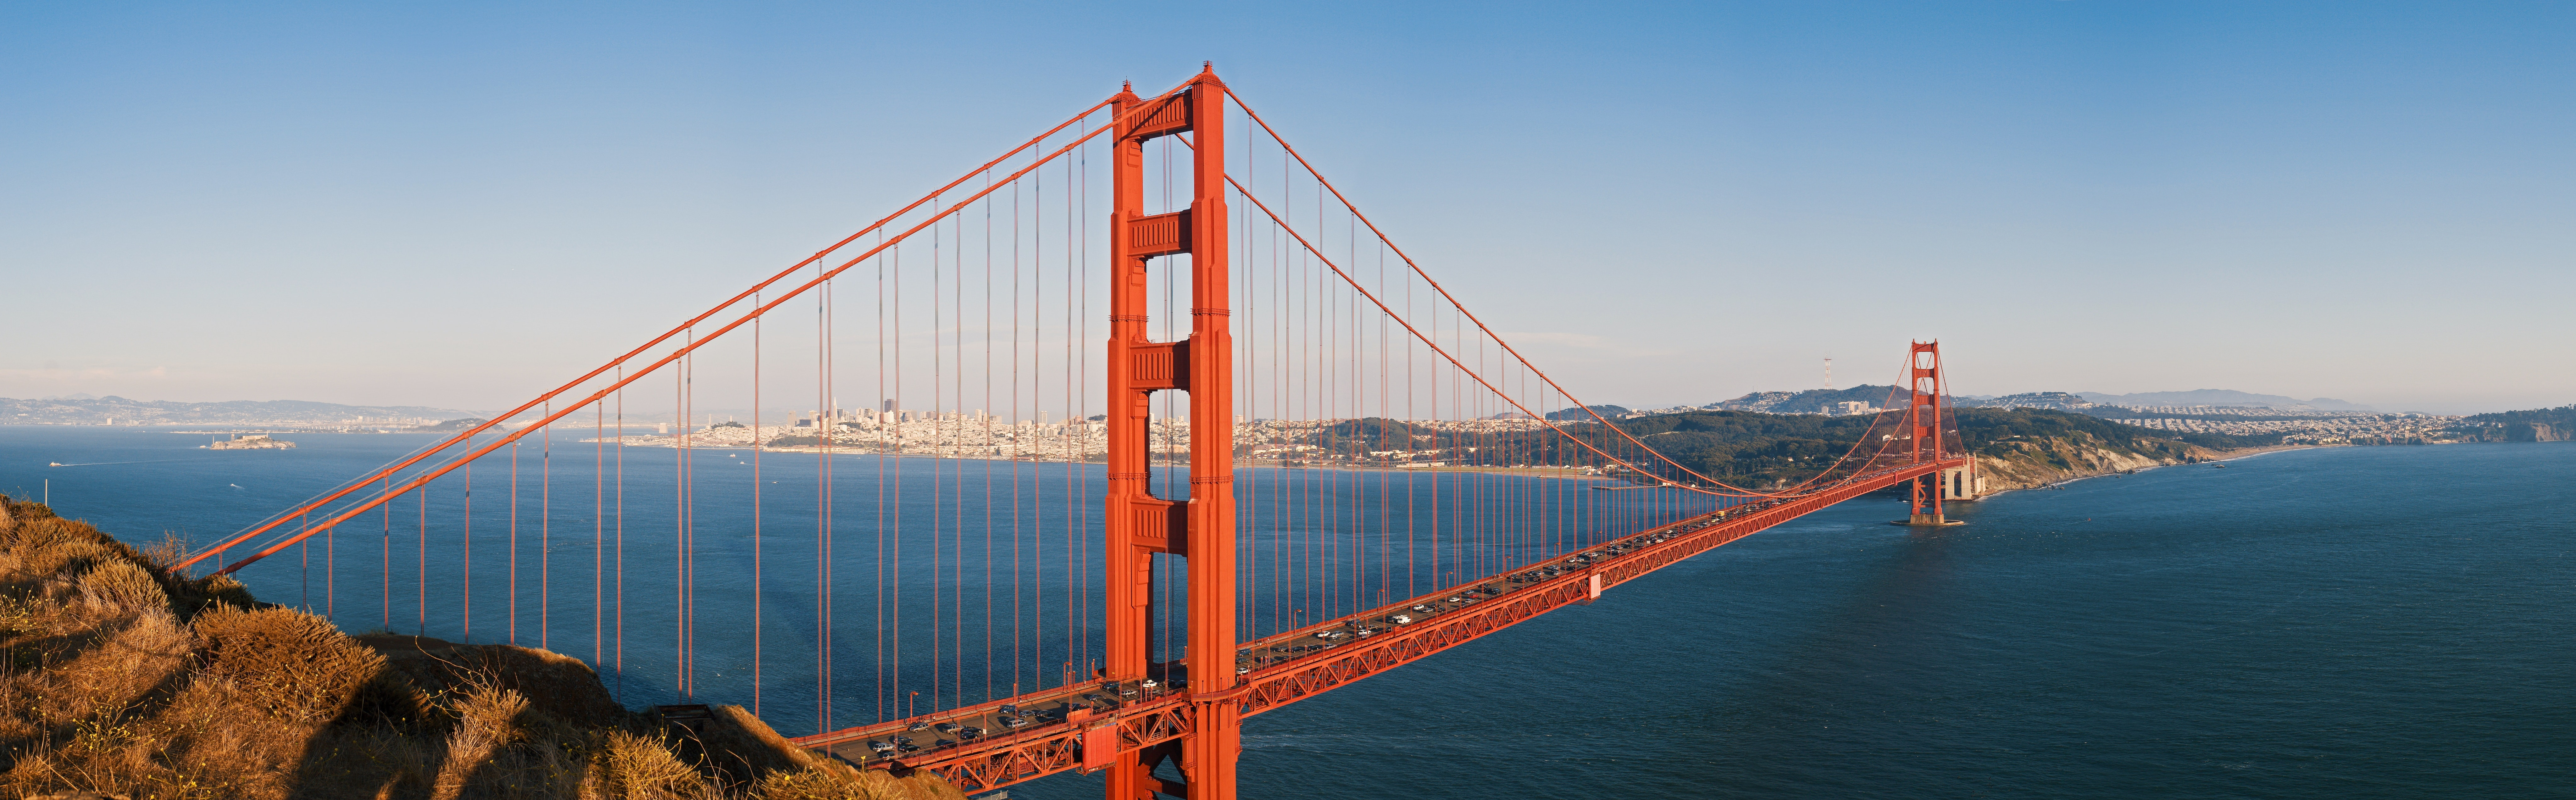
\includegraphics[scale=.5]{../data/content_bridge}
						\caption{Content Image}
					\end{minipage}\hfill
				\end{figure}
				
				\begin{figure}[htb!]
					\begin{minipage}{1\textwidth}
						\centering
						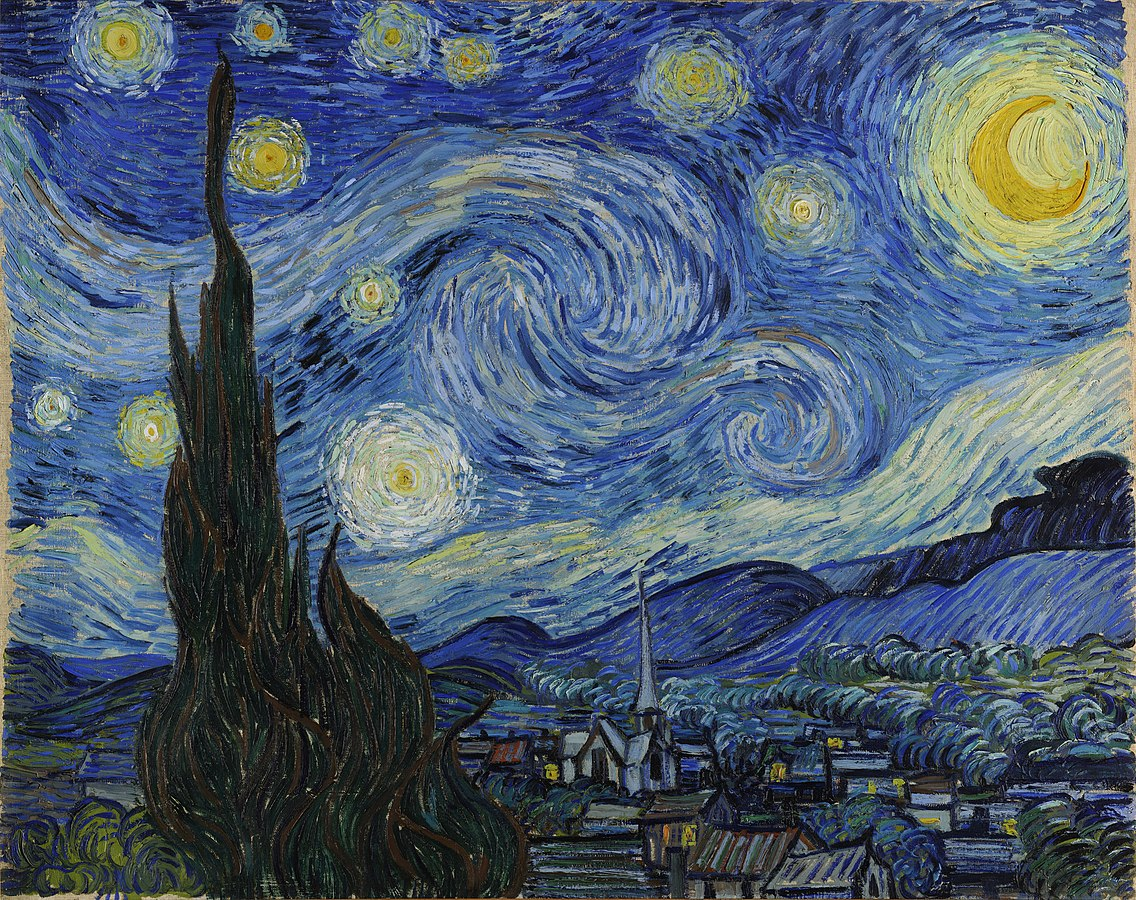
\includegraphics[scale=.2]{../data/style_vangogh}
						\caption{Style image 1}
					\end{minipage}\hfill
				\end{figure}
				
				\begin{figure}[htb!]
					\begin{minipage}{1\textwidth}
						\centering
						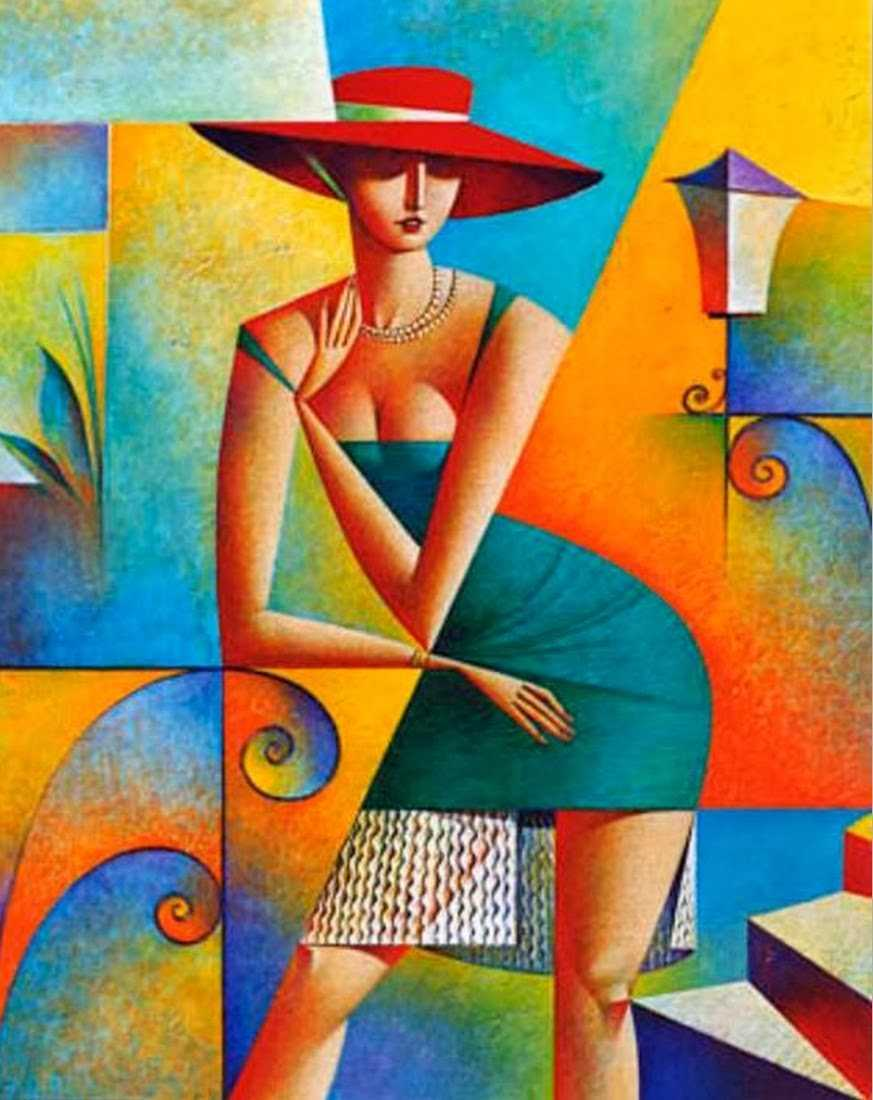
\includegraphics[scale=.2]{../data/style_mujer}
						\caption{Style Image 2}
					\end{minipage}\hfill
				\end{figure}
			

				Parámetros:
				\begin{itemize}
					\item Ts: Índice de las capas elegidas para extraer el estilo
					\item Tc: Índice de las capas elegidas para extraer el contenido
					\item Ws: Peso asignado al estilo
					\item Wc: Peso asignado al contenido
					\item N: Si está seleccionado, indica que he utilizado la imagen de contenido con ruido como imagen inicial
					\item avg: Si está seleccionado, indica que he utilizado avg pooling en vez de max pooling en la VGG
					\item size: dimensiones utilizadas para las imágenes 
				\end{itemize} 
				
				\begin{longtable}{| m{2.5cm} | m{0.5cm} | m{1.2cm} | m{0.5cm} | m{0.5cm} | m{1cm} | m{1.6cm} | c |}
					\hline
					\multicolumn{1}{|c|}{Ts} & \multicolumn{1}{c|}{Tc} & \multicolumn{1}{c|}{Ws} & \multicolumn{1}{c|}{Wc} & \multicolumn{1}{c|}{N} & \multicolumn{1}{c|}{avg} & \multicolumn{1}{c|}{size } & image  \\ \hline
					2,4,8,12,16                         & 9                                   & 500                               & 5                                   &                                    &                               & 224x224                         & 
					\begin{minipage}{.3\textwidth}
						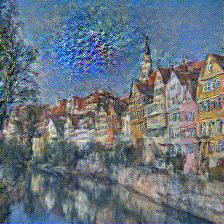
\includegraphics[width=1\linewidth, height=50mm]{pics/image2}
					\end{minipage} \\
					 
					2,4,8,12,16                         & 9                                   & 100000                            & 1                                   &                                    &                               & 224x224                         & 
					\begin{minipage}{.3\textwidth}
						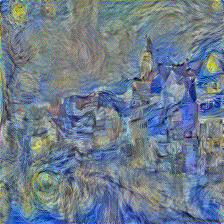
\includegraphics[width=1\linewidth, height=50mm]{pics/image5}
					\end{minipage} \\
					1,3,5,9,13                          & 3                                   & 100000                            & 1                                   &                                    &                               & 224x224                         & 
					\begin{minipage}{.3\textwidth}
						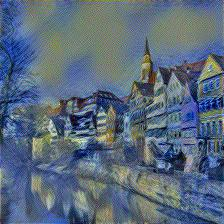
\includegraphics[width=1\linewidth, height=50mm]{pics/image1}
					\end{minipage} \\
					1,3,5,9,13                          & 10                                  & 500                               & 1                                   &                                    & x                             & 224x224                         & 
					\begin{minipage}{.3\textwidth}
						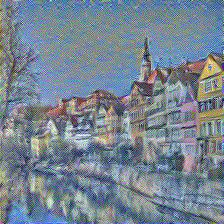
\includegraphics[width=1\linewidth, height=50mm]{pics/image3}
					\end{minipage} \\
					2,4,8,12,16                         & 9                                   & 100000                            & 1                                   & x                                  & x                             & 224x224                         & 
					\begin{minipage}{.3\textwidth}
						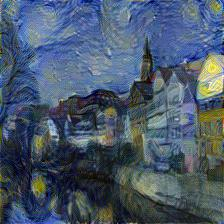
\includegraphics[width=1\linewidth, height=50mm]{pics/image4}
					\end{minipage} \\
					2,4,8,12,16                         & 9                                   & 100000                            & 1                                   & x                                  & x                             & 512x512                         & 
					\begin{minipage}{.3\textwidth}
						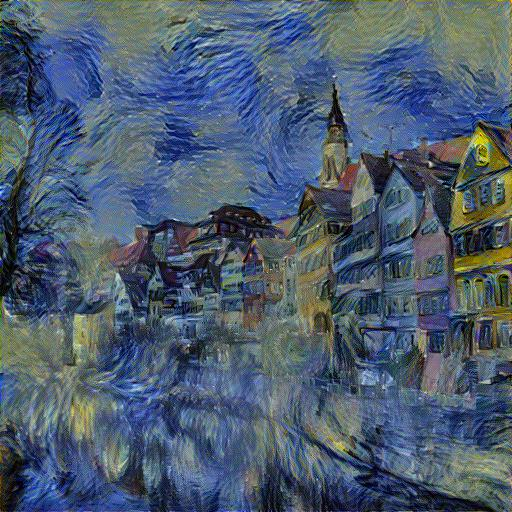
\includegraphics[width=1\linewidth, height=50mm]{pics/image6}
					\end{minipage} \\
					2,4,8,12,16                         & 9                                   & 100000                            & 5                                   & x                                  & x                             & 512x512                         & 
					\begin{minipage}{.3\textwidth}
						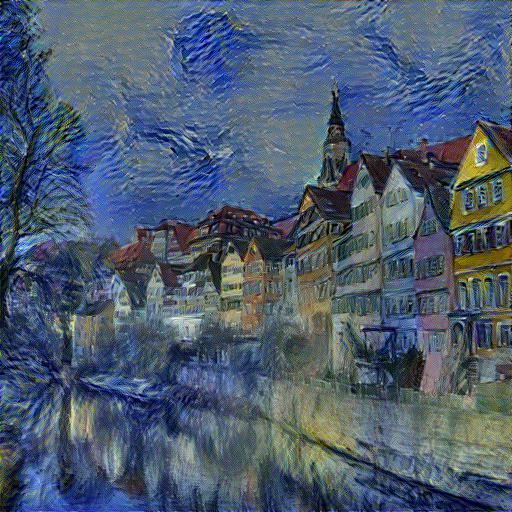
\includegraphics[width=1\linewidth, height=50mm]{pics/image7}
					\end{minipage} \\
					1,3,5,9,13                          & 9                                   & 100000                            & 2                                   & x                                  & x                             & 512x512                         & 
					\begin{minipage}{.3\textwidth}
						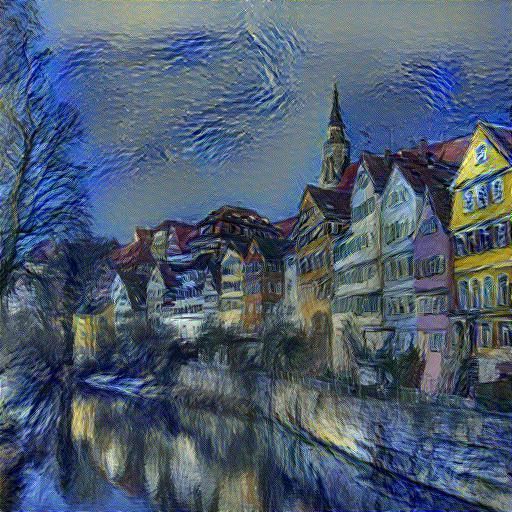
\includegraphics[width=1\linewidth, height=50mm]{pics/image8}
					\end{minipage} \\
					2,4,8,12,16                         & 9                                   & 100000                            & 5                                   & x                                  & x                             & 512x512                         & 
					\begin{minipage}{.3\textwidth}
						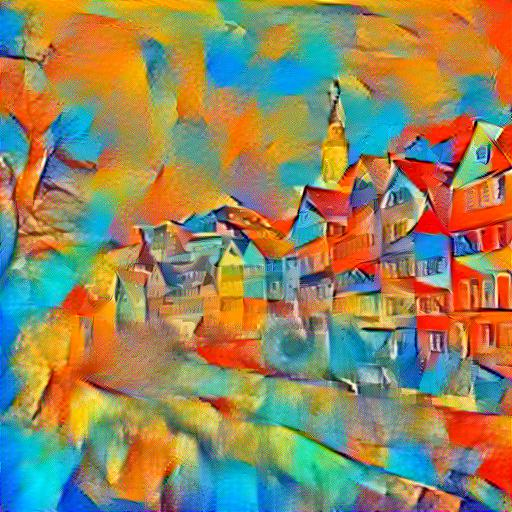
\includegraphics[width=1\linewidth, height=50mm]{pics/image9}
					\end{minipage} \\ \hline
				\end{longtable}
   		
   			Como podemos observar, los mejores resultados se obtienen con un style weight muy alto (100000), utilizando avg pooling y con dimensiones de imagen altas.
    
\begin{thebibliography}{50}
	\bibitem{neural-paper} 
	\href{https://arxiv.org/pdf/1508.06576.pdf}{A Neural Algorithm of Artistic Style}
\end{thebibliography}

\end{document}